
\section{Cross-point ReRAM Macro Design??}\label{sec:macro}
Since the array size of a cross-point ReRAM array is strictly limited by
reliability requirements, the design of a ReRAM macro is greatly different
from the traditional DRAM design. A cross-point ReRAM macro is implemented
by establishing a large amount of small cross-point arrays with
appropriate peripheral circuity and organizations. In this section, we
evaluate the area, energy consumption, and bandwidth of a 256 Mbits ReRAM
macro. We apply the similar memory organization as Kawahara's
work~\cite{crossbar_Panasonic}. The 256 Mbits ReRAM macro consists of
eight planes, each of which is 32 Mbits. Each plane has separate wordline
decoder, bitline selectors, sense amplifiers, and write circuity. Due to
limitations of space, we only present the results of ReRAM macro
implemented by four different typical cell parameters: ($Kr=20,
I_w=40uA$), ($Kr=20, I_w=200uA$), ($Kr=40, I_w=40uA$), and ($Kr=40,
I_w=200uA$). For each of them, we vary the number of bit per write to
investigate the relation among the area, energy consumption, and bandwidth
of the ReRAM macro.


Figure~\ref{}
\begin{figure}[!t]
\centering\label{table}
  % Requires \usepackage{graphicx}
  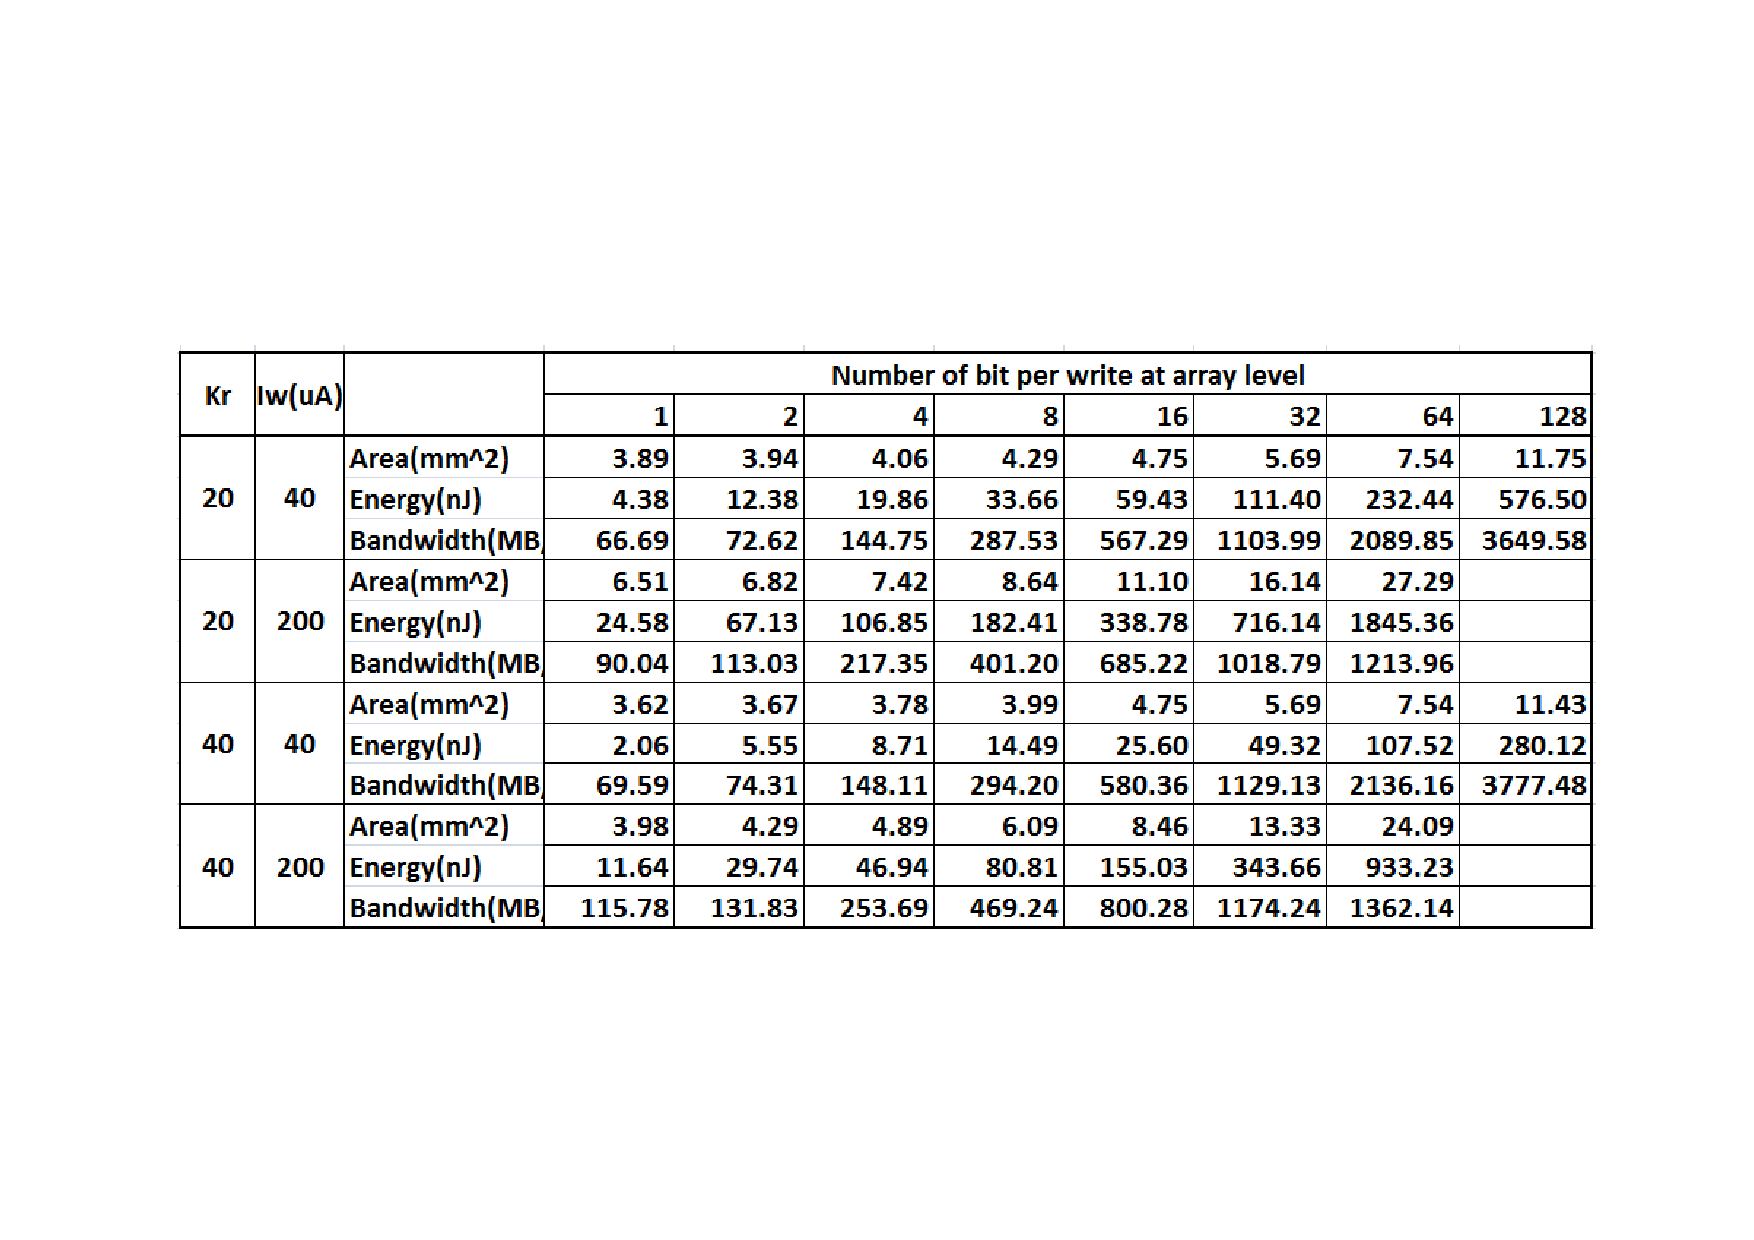
\includegraphics[width=0.5\textwidth]{./figures/Table}\\
  \caption{Area, energy, and bandwidth results of 256 Mbits ReRAM macro.}
  \vspace{-5pt}
\end{figure}


\begin{figure}[!t]
\centering\label{EpJ}
  % Requires \usepackage{graphicx}
  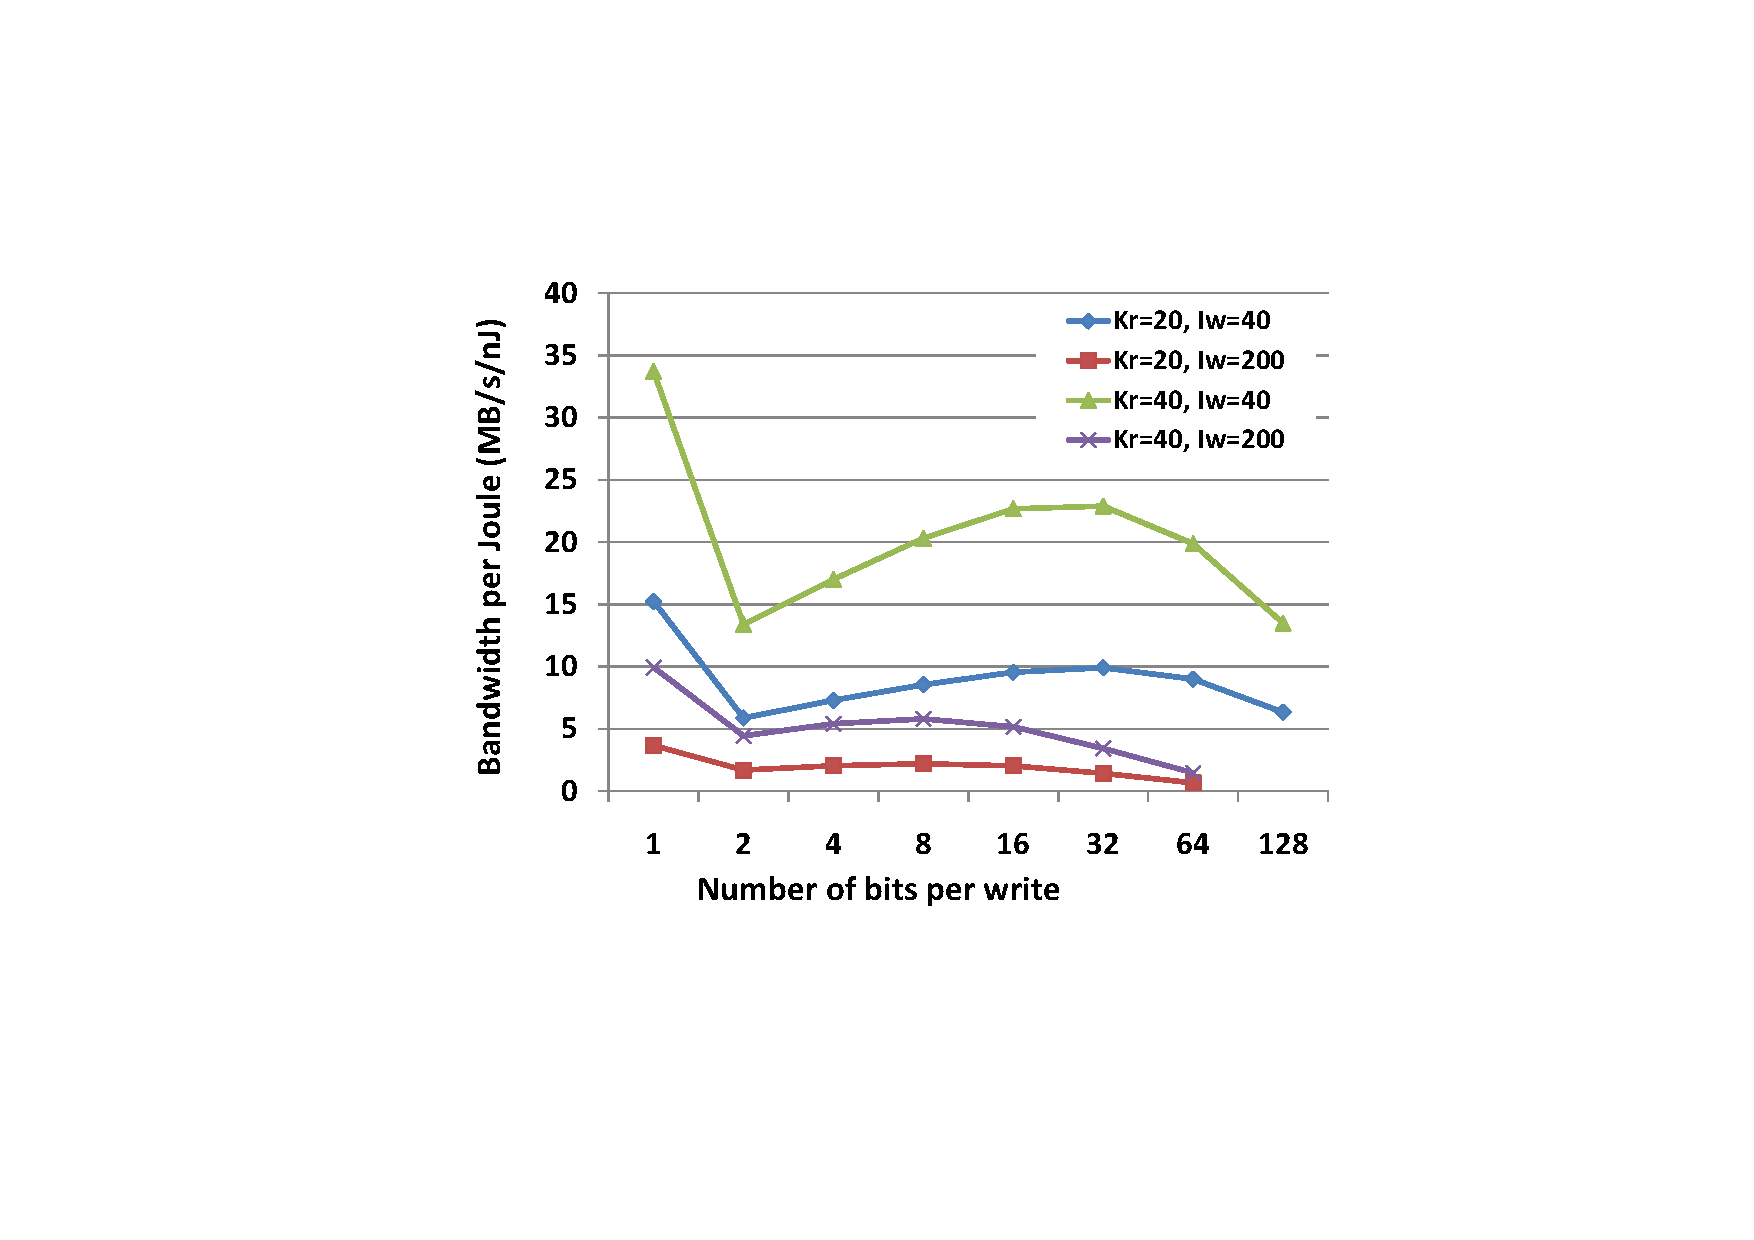
\includegraphics[width=0.4\textwidth]{./figures/EpJ}\\
  \caption{Bandwidth per Joule of 256 Mbits ReRAM macro.}
  \vspace{-5pt}
\end{figure}

%\begin{table}
%\begin{tabular}{|l|l||l|l|l|l|l|l|l|l|}
%\hline
%\multicolumn{8}{|c|}{Num of bit per write}\\
%$Kr$ & $I_w$ & 1 & 2 & 4 & 8 & 16 & 32 & 64 & 128 \\\hline
%\multirow{3}{*}{20} & \multirow{3}{*}{20} & & ~ & ~ & ~ & ~ & ~ & ~ & ~ & ~ \\
%& ~ & ~ & ~ & ~ & ~ & ~ & ~ & ~
%& ~ & ~ & ~ & ~ & ~ & ~ & ~ & ~\\\hline
%20 & ~ & ~ & ~ & ~ & ~ & ~ & ~ & ~ & ~ \\\hline
%20 & ~ & ~ & ~ & ~ & ~ & ~ & ~ & ~ & ~ \\\hline
%20 & ~ & ~ & ~ & ~ & ~ & ~ & ~ & ~ & ~ \\\hline
%40 & ~ & ~ & ~ & ~ & ~ & ~ & ~ & ~ & ~ \\\hline
%40 & ~ & ~ & ~ & ~ & ~ & ~ & ~ & ~ & ~ \\\hline
%40 & ~ & ~ & ~ & ~ & ~ & ~ & ~ & ~ & ~ \\\hline
%40 & ~ & ~ & ~ & ~ & ~ & ~ & ~ & ~ & ~ \\\hline
%40 & ~ & ~ & ~ & ~ & ~ & ~ & ~ & ~ & ~ \\\hline
%40 & ~ & ~ & ~ & ~ & ~ & ~ & ~ & ~ & ~ \\\hline
%40 & 200 & ~ & ~ & ~ & ~ & ~ & ~ & ~ & ~ \\
%\end{tabular}
%\end{table}
